
\documentclass{amsart}

\usepackage{graphicx}
%\usepackage[altbullet]{lucidabr}
%two lines below change font (font intalled manually (i.e. uploaded))
%\usepackage{fontspec}
%\setmainfont[Ligatures=TeX]{LucidaBrightRegular.ttf}
%\usepackage{kpfonts}    % for nice fonts
% option [light] for more aery documents
\usepackage{color}  %for color of references
\usepackage[dvipsnames]{xcolor} %for color of references
\usepackage{caption}
\usepackage{fancyhdr}
\usepackage[pagebackref,colorlinks, citecolor=BlueViolet,urlcolor=BlueViolet]{hyperref}
\hypersetup{colorlinks = BlueViolet, allcolors = BlueViolet}
\usepackage[nameinlink,noabbrev]{cleveref} 
\usepackage{natbib}
\usepackage{multicol}
\usepackage{multirow}
%\usepackage{lscape}
\usepackage{pdflscape}
\usepackage{amssymb}
\usepackage{geometry}
\usepackage{longtable}
\usepackage{colortbl}
\usepackage{dsfont}
\usepackage{bm}
\usepackage{mathtools}
\usepackage{pgf}
\usepackage{tikz}
\usepackage{soul}
\usepackage{tikz}
\usepackage{tikz,fullpage}
\usepackage{pgf}
\usepackage{tikz}
\usepackage{bbm} %for the indicator function
\usetikzlibrary{shapes.geometric, arrows} %to create flow charts
\usepackage{bold-extra} %for bold small caps in the title
\usepackage{dirtree} % to create lists as tree

%\renewcommand{\familydefault}{\sfdefault} %for the sans serif font

%AMS original setup for mathematical elements
\newtheorem{theorem}{Theorem}[section]
\newtheorem{lemma}[theorem]{Lemma}
\theoremstyle{definition}
\newtheorem{definition}[theorem]{Definition}
\newtheorem{example}[theorem]{Example}
\newtheorem{xca}[theorem]{Exercise}
\theoremstyle{remark}
\newtheorem{remark}[theorem]{Remark}
\numberwithin{equation}{section}

%    Absolute value notation
\newcommand{\abs}[1]{\lvert#1\rvert}

%    Blank box placeholder for figures (to avoid requiring any
%    particular graphics capabilities for printing this document).
\newcommand{\blankbox}[2]{%
  \parbox{\columnwidth}{\centering
%    Set fboxsep to 0 so that the actual size of the box will match the
%    given measurements more closely.
    \setlength{\fboxsep}{0pt}%
    \fbox{\raisebox{0pt}[#2]{\hspace{#1}}}%
  }%
}

%Tikz setup for a flow chart
\tikzstyle{modelblock} = [rectangle, rounded corners, minimum width=3cm, minimum height=1cm,text centered, draw=black, fill=white, text ragged]

\tikzstyle{arrow} = [thick,->,>=stealth]

\begin{document}

\title{EC539 - Referee report}

%    Information for first author
\author{Arnaud Dy\`evre}
%\address{}
%\curraddr{}
%\email{a.dyevre@lse.ac.uk}
%\thanks{}

%    Information for second author
%\author{}
%\address{}
%\email{}
%\thanks{}

%    General info
%\subjclass[2000]{}

%\date{\today. First created October 19, 2019}

%\dedicatory{}
%\keywords{}

%\begin{abstract}

%\end{abstract}

\maketitle

\begin{center}
\end{center}


\vspace{12pt}

Referee report of the journal article: \\ 
\textbf{Kiyotaki, N., \& Moore, J.} (2019). ``Liquidity, business cycles, and monetary policy''. \textit{Journal of Political Economy}, 127(6), 2926-2966.

%% The correct journal style for \specialsection is all uppercase; a known bug
%% in amsart.cls prevents this, so input must be uppercase until it is fixed.
%\specialsection*{This is a Special Section Head}
%\specialsection*{THIS IS A SPECIAL SECTION HEAD}
%This is an example of a special section head%
%%%%%%%%%%%%%%%%%%%%%%%%%%%%%%%%%%%%%%%%%%%%%%%%%%%%%%%%%%%%%%%%%%%%%%%%
%\footnote{Here is an example of a footnote. Notice that this footnote text is running on so that it can stand as an example of how a footnote with separate paragraphs should be written.
%\par
%And here is the beginning of the second paragraph.}%
%%%%%%%%%%%%%%%%%%%%%%%%%%%%%%%%%%%%%%%%%%%%%%%%%%%%%%%%%%%%%%%%%%%%%%%%
\newpage 

\subsection*{Summary of the paper} This article is an ambitious theoretical exploration of how liquidity constraints can explain co-movements in asset prices and real quantities. Its main contribution is the introduction of a limit on the sale of equity in the budget constraint of investing entrepreneurs. The model is able to generate a rich set of (large) responses in capital utilisation, in output and in the price of assets in spite of its simplicity. The most sophisticated environment presented in the paper simply consists of entrepreneurs-investors, entrepreneurs-savers, workers, and a rule-based central banker. Workers consume their wage. Entrepreneur-savers produce outputs, do not have an investment opportunity and lend to entrepreneurs-investors. Entrepreneur-investors liquidate equity and borrow funds from entrepreneur-savers to finance investment opportunities, subject to a liquidity+borrowing constraint. Finally, the central bank exchanges illiquid equity for liquid equity (=money). One may describe their model as ``LBC''--liquidity business cycle. I summarise the model graphically below.

\subsubsection*{Summary of the full model} Given an aggregate state $\left(K_{t}, Z_{t}, N_{t}^{g}, a_{t}, \phi_{t}\right)$, and an exogenous law of motion for $\left(a_{t}, \phi_{t}\right)$, the model satisfies the following conditions:

\begin{tikzpicture}[->, node distance=cm, 
blocklarge/.style ={rectangle, rounded corners, draw=black, fill=white,  text centered, text width=27em},
blockvlarge/.style ={rectangle, rounded corners, draw=black, fill=white,  text centered, text width=34em},
blockmed/.style ={rectangle, rounded corners, draw=black, fill=white,  text centered, text width=22em},
blockmonetary/.style ={rectangle, rounded corners, draw=black, fill=white,  text centered, text width=17em},
block/.style ={rectangle, rounded corners, draw=black, fill=white,  text centered, text width=14em},
blockredlarge/.style ={rectangle, draw=red, fill=white,  text centered, text width=20em},
blockblue/.style ={rectangle, rounded corners, draw=blue, fill=white,  text centered, text width=16em}]
%, minimum height=4em

\node (workers) [blockvlarge] {\textbf{Workers} (unit mass) \\
$$\max_{(C_t^w, L_t, N_{t+1}^w, M_{t+1}^w)} E_{t} \left[ \sum_{s=t}^{\infty} \beta^{s-t} U\left(C_{s}^{w}-\frac{\omega}{1+\nu}\left(L_{s}\right)^{1+\gamma}\right) \right]$$ \\
$$\mathrm{s.t.} \quad C_{t}^{w}+q_{t} \textcolor{blue}{\underbrace{\left(N_{t+1}^{w}-\lambda N_{t}^{w}\right)}_{= 0 \textrm{ in equilibrium}}}+p_{t}\textcolor{blue}{\underbrace{\left(M_{t+1}^{w}-M_{t}^{w}\right)}_{0}} + \textcolor{ForestGreen}{\underbrace{(\beta z_{t+1} - \sigma z_{t+1})}_{\textrm{storage}}}=w_{t} L_{t}+r_{t} \textcolor{blue}{\underbrace{N_{t}^{w}}_{0}}$$
$$ N_{t+1}^{w} \textcolor{blue}{=} \left(1-\phi_{t}\right) \lambda N_{t}^{w} \textcolor{blue}{=} 0 $$
$$ M_{t+1}^{w} \textcolor{blue}{=} 0 $$
};

\node (entrepreneurs) [block, below of=workers, yshift=-3.8cm] {\textbf{Entrepreneurs} (unit mass) \\
$$ \max_{\ell_t} A_{t} k_{t}^{\gamma} \ell_{t}^{1-\gamma}-w_{t} \ell_{t} -r_{t} k_{t}$$
};

\node (investing_entrepreneurs) [blockmed, below of=entrepreneurs, yshift=-3.8cm, xshift=-4.5cm] {\textbf{Investing Entrepreneurs} \\
Get investment opportunity with probability $\textcolor{red}{\pi}$
$$ \max_{c_t^i, \textcolor{red}{i_t}^i, n_{t+1}^i, m_{t+1}^i} E_{t} \sum_{s=t}^{\infty} \beta^{s-t} u\left(c_{s}^i\right)$$
$$\mathrm{s.t.} \quad c_{t}^i+\textcolor{red}{i_{t}^i}+q_{t}\left(\Delta n_{t}^i-\textcolor{red}{i_{t}^i}\right)+p_{t}\left(\Delta m_{t}^i\right) + \textcolor{ForestGreen}{\underbrace{(\Delta z_t^i)}_{\textrm{storage}}} =r_{t} n_t^i$$
$$ n_{t+1}^i \geq \textcolor{red}{(1-\theta) i_{t}^i}+\left(1-\phi_{t}\right) \lambda n_{t}^i$$
$$m_{t+1}^i \geq 0$$
$$k_{t+1}^i=\lambda k_{t}^i+\textcolor{red}{i_{t}^i}$$ 
};

\node (noninvesting_entrepreneurs) [blockmed, below of=entrepreneurs, yshift=-3.8cm, xshift=4.5cm] {\textbf{Non-investing Entrepreneurs} \\
$$ \max_{c_t^s, n_{t+1}^s, m_{t+1}^s} E_{t} \sum_{s=t}^{\infty} \beta^{s-t} u\left(c_{s}^s\right)$$
$$\mathrm{s.t.} \quad c_{t}^s+q_{t}\left(\Delta n_{t}^s-\lambda \right)+p_{t}\left(\Delta m_{t}^s\right) + \textcolor{ForestGreen}{\underbrace{(\Delta z_t^s)}_{\textrm{storage}}} =r_{t} n_t^s$$
$$ n_{t+1}^s \geq \left(1-\phi_{t}\right) \lambda n_{t}^s$$
$$m_{t+1}^s \geq 0$$
$$k_{t+1}^s=\lambda k_{t}^s$$ 
};

\node (policy) [blockmonetary, below of=investing_entrepreneurs, xshift=2cm , yshift= -4.5cm] {\textbf{Monetary policy} \\
$$\frac{N_{t+1}^{g}}{K}=\psi_{a} \frac{a_{t}-a}{a}+\psi_{\phi} \frac{\phi_{t}-\phi}{\phi}$$
$$\mathrm{s.t.} \quad q_{t}\left(\Delta N_{t}^{g}\right) = r_{t} N_{t}^{g}+ p_t (M_{t+1} - M_t)$$
};

\node (clearing) [blockblue, right of=policy, xshift= 8cm] {\textbf{Market clearing} \\
Labour: $L_t = \ell_t$ \\
Goods: $y_t  = C^w_t + c^i_t + c^s_t + i_t^i + Z_t$\\
Equity: $n^i_t + n^s_t + N^g_t + N^w_t= K_t$\\
Money: $m^i_t + m^s_t + M^g_t + M^w_t = M_t$\\
};

\path[every node/.style={font=\sffamily\small}]
    (entrepreneurs) edge node [right] {$r_t^*$} (investing_entrepreneurs)
    (entrepreneurs) edge node [right] {$r_t^*$} (noninvesting_entrepreneurs)
    (workers) edge [bend right] node [left] {$\ell_t$} (entrepreneurs)
    (entrepreneurs) edge [bend right] node [left] {$w_t^*$} (workers)
    (noninvesting_entrepreneurs) edge [bend right] node [below] {$q_t^*$} (investing_entrepreneurs)
    (noninvesting_entrepreneurs) edge [bend right=20] node [below] {$p_t^*$} (investing_entrepreneurs)
    (investing_entrepreneurs) edge [bend right] node [above] {$n_t$} (noninvesting_entrepreneurs)
    (investing_entrepreneurs) edge [bend right=20] node [above] {$m_t$} (noninvesting_entrepreneurs)
    (policy) edge node [left] {CB exchanges $m_t^i$ for $n_t^i$} (investing_entrepreneurs)
    (investing_entrepreneurs) edge node [right] {(at market prices)} (policy)
    (noninvesting_entrepreneurs) edge node [right] {CB exchanges $m_t^s$ for $n_t^s$ (at market prices)} (policy)
    (policy) edge node [right] {} (noninvesting_entrepreneurs)

    %(3) edge node [right] {} (4)
    %(4) edge[bend right] node [left] {} (1);

%\draw [arrow] (workers) -- node {$\quad \quad \ell_t^*$}(entrepreneurs)
%\draw [arrow] (entrepreneurs) -- node {$w_t^*$}(workers)
%\draw [arrow] (entrepreneurs) -- node {}(investing_entrepreneurs)

\end{tikzpicture}


\subsubsection*{Main takeaways} In a ``monetary economy'' described above, the liquidity constraint has five important consequences: (i) it prevents the economy to reach its first best allocation of capital, (ii) there is a gradient of rates of return,\footnote{Money provides a higher return than  equity if one has an investment opportunity next period, but less if one does not.} (iii) it leads entrepreneurs to hold precautionary money for no other reason than weathering times when they are illiquid, (iv) a cheap storage technology will divert resources away from capital investment, and (v) monetary policy of the Quantitative Easing type reduces the impact of an illiquidity shock on consumption, investment, output, and the price of equity.\\

Two parameters and two types of assets lie at the heart of the model. With regards to parameters; $\theta$ is the share of future earnings from the new capital an entrepreneur can credibly pledge, and $\phi$ is the share of equity they can convert into investable funds. Low $\theta$ and $\phi$ mean tight asset-based borrowing and liquidity constraints, respectively. The important assets are money, which is liquid but provide a low return, and equity, whose liquidity is determined by $\phi$ and which provides a return $r_t$. \\

The authors provide numerical examples of dynamic impulse responses to liquidity and productivity shocks. They compare models without storage or monetary policy to the full model.\\

\subsection*{Major comments} 

\subsubsection*{Theoretical relevance} The paper is an important effort to explicitly include liquidity constraints in a business cycle model. Until the Great Recession, most RBC models ignored the impact of liquidity constraints on aggregate economic activity \citep{gertler2010financial}. The traditional approach to credit friction has been to model entrepreneurs as being able to credibly pledge only a limited share of their future gains, or to collateralise only part of their current capital. For instance, canonical models such as \cite{bernanke1989agency} and \cite{kiyotaki1997credit} endogenise financial market frictions faced by actors in the real economy by creating an agency problem between lenders and borrowers. As a borrower's balance sheet deteriorates, their access to external finance becomes limited and they must bear most of the risk of the investment project with internal funds. The two-way interaction between investment and capital on the one hand, and access to credit on the other amplifies credit shocks. With the notable exception of \cite{holmstrom1997financial}, no macro-finance paper had thoroughly studied the theoretical implication of liquidity shortages in the financial sector before this one.\\

Its second notable theoretical contribution is to generate substantial and long-lived responses in output, consumption, investment, equity price and capital utilisation without relying on implausibly large exogenous shocks like standard RBC models. In the seminal \cite{kiyotaki1997credit} paper, the asset price moves little after a technology shock: it rises by 0.37\% following a 1\% increase in productivity. In comparison, the price of money and the price of equity in \cite{kiyotaki2019liquidity} rise by 1.6 and 0.9\% respectively after the same shock. The liquidity constraint also plays a key role in generating large response in consumption. without it binding, consumption would depend on permanent income rather than current income.\\

\subsubsection*{Need for justifications of some modelling choices} However, while the responses to shocks are large, some authors have stressed that the choices of functional forms for utility and production matter a great deal to determine the magnitude of these responses. \cite{cordoba2004credit}, for instance, find that under concave preferences, concave technology and collateralised debt, borrowing constraints can indeed amplify shocks, but these amplifications are relatively small. Large amplifications can be obtained under implausible parameter values, or worse, the equilibrium is not saddle path. More sensitivity analyses would have been welcome to assess wether these criticisms apply to liquidity constraints as well.\\

Lastly, more justification about the specific magnitude of the drop in liquidity in the numerical exercise would have been helpful. The authors use a drop in resaleability of equity from 20\% to 6\%.  It is hard for the reader to know if this drop is large or small. Back-of-the-envelope calculations can help putting these results in perspective: a 20\% resaleability constraints means that it takes 3.1 quarters for an entrepreneur to liquidate half of their equity (conditional on them having investment opportunties in every period). It takes 11.2 quarters when $\phi = 0.06$ instead. As this seems to be a very long period for liquidation (longer than the Great Recession in the U.S.), some comparison with real data would have helped to put this number in context.\\

\subsubsection*{Empirical/policy relevance} Quantitatively, the unorthodox policies carried out by Central Banks in Europe, America and England in the wake of the 2008 crisis amounted to a lot of liquidities. The Fed for instance added US\$1.5 trillion worth of assets to its balance sheet in early 2009 (see Figure \ref{fig:fedsheet}). In this respect, having a clear theoretical understanding of how new liquidity helped keep the financial sector afloat is paramount. It is worth noting, that when the thought of injecting money into the economy by buying off illiquid asset was first formulated by Kiyotaki and Moore as part of Moores's 2001 \textit{Clarendon Lectures}, the idea was deeply unconventional \citep{kiyotaki2001liquidity}. The Great Recession has been a spectacular confirmation of their vision. The policy implications are evident with the hindsight of the Great Recession: the liquidity of assets being traded by banks matter, and fluctuations in liquidity may trigger economic recessions.\\

\subsubsection*{Modelling the financial sector/endogenising the liquidity constraint} A notable omission of the paper is the absence of the financial sector as an optimising agent. In Kiyotaki and Moore's model, the liquidity shock is simply an exogenous Markov process $\lambda_t$. Modelling the mechanisms through which liquidity constraints emerge would have been an engaging addition to the paper. This would understandably complicate the model as the shocks generating tighter liquidity constraints could take multiple forms; a sudden drop in trust in the inter-bank market, the removal of a particular class of assets from the market, or regulatory changes for instance. Modelling liquidity contractions as a stochastic risk allows them to remain agnostic about their origin. Yet, putting some behavioural structure on how the financial sector would react to these underlying shocks could have painted a more comprehensive picture of liquidity-induced recessions. See \cite{he2013intermediary, angeloni2013capital, gertler2010financial} for recent work doing just this.

%A related point In particular, it would have been nice to endogenise the agency problem created by the emergence of the central bank as a lender of last resort. Liquidity crises could be triggered by banks taking risky positions on the asset side of theuir balance sheet, under the assumption that they would be rescued by the government/the central bank.\\

%More fundamentally, my critique of the paper would be to treat the drop in liquidity as fully endogenous, and the liquidity constraint as fully reduced-form: dose-response? What make the liquidity of some asset change?\\
\subsection*{Minor comments}

\subsubsection*{Making sense of the entrepreneur-savers} While the model is impressive in capturing many aspects of the last economic crisis, the assumption that funds used by entrepreneurs-investors come from entrepreneurs who do not have an investment opportunity would have deserved more justification. It does not seem to fit in with the way corporate credit works. A more credible assumption would have been to make workers lend to firms, as depositors. The authors could have accommodated this aspect by using overlapping generations for the workers: the first generation consumes its wage, while the second saves. Here again, modelling the endogenous response of the financial sector to the supply of funds could have helped. \\ 

\subsubsection*{Distributional consequences of QE} The model's parsimony is one of its strengths, but I wonder how much interesting heterogeneity is hidden behind the representative agent assumption. A critique of the QE-type policies carried out by the ECB and the Fed after the 2008 crisis was that it surely helped financial institutions and kept the banking system afloat, but it also increased the gap between the wealthiest and the poorest.\footnote{Adding heterogenity in previous-period wealth of labour income would however make the model much more complicated. I can understand why the authors kept it so streamlined.}

%Furthermore, the Fed, the ECB, the Bank of England and many other large central banks engaged in unconventional policies that involved some form of direct lending in credit markets. The policy channel modelled by the authors is a direct theoretical counterpart to the Fed's expansion of the discount window loans, the Troubled Asset Relief Program, and the emergency loans to J.P. Morgan Chase (who absorbed Bear Stearns) and AIG.\\

%\subsubsection*{Obtaining a quantitatively large response in numerical simulations} Question the choice of preferences and technology. Are they linear? And if yes would the shock propagate similarly if these preferences were more traditional? 

%Even in the simplest version of the model, the liquidity constraint amplifies the impact of a productivity shock on aggregate consumption: without the binding liquidity constraint consumption would depend on permanent income rather than current income (see Figure 1 of the paper). But some authors have argued that liquidity constraints are not that powerful of a mechanism in amplifying productivity shocks \citep{cordoba2004credit}. It should be noted that th \\


\subsection*{Suggested extension}

\subsubsection*{Benchmarking}
I believe the paper would have benefited from a model more directly applicable to monetary policy. Considering the importance of the liquidity channel in explaining important recent crises (Great Recession, the Greek debt crisis), a comparison of the model performance with that of the the New Keynesian canon \citep{gali2015monetary} would have helped the reader to assess its merits.\\

%A lack of liquidity. The contagion of the recent financial crisis to the broader real economy. But are these liquidity constraints quantitatively big? \cite{liu2013land} have developed a DSGE model with land as a collateral asset and shocks driving most of the fluctuation in land prices. Their model is motivated by the fact that business investment dropped in tandem with land prices in the U.S. at the onset of the Great Recession.\\

The model clearly describes the channel through which unorthodox monetary policy can dampen illiquidity-induced recessions. Yet the effectiveness of this type of policy is mostly an empirical question. In this respect, I see this article as a first step in understanding the impact of liquidity constraints on asset prices and quantities. More needs to be done to quantify how important this cause of recession is. \cite{del2017great} and co-authors have done such work, it would be interesting to see more emprical confirmation of Kiyotaki and Moore's framework. \\


%\textbf{see if possible to include this...}
%Secondly, In general, DSGE models with credit constrained households manage to explain co-movements between house prices and consumption expenditures. But they have a hard time delivering co-movement between land prices and business investment \citep{iacoviello2010housing}. KM delivers this by assuming that entrepreneurs--rather than households/workers--are credit constrained. See \cite{liu2013land} for . The causal channel in both models is: a positive shock to land price raises firms' borrowing capacity, which in turns facilitates an expansion in investment and production. While this channel intuitively makes sense, the empirical study of \cite{lian2019anatomy} suggests that 83\% of large U.S. firms' corporate debt is based on cash flow from their operations (80\% in aggregate). It would thus have been helpful to show how important cash-flow-based debt is in Kiyotaki and Moore's model, compared to the liquidity and the investment-based (=future asset-based) borrowing constraints. One can think of a modified version of constraint (5) in their paper: $$n_{t+1} \geq(1-\theta) i_{t}+\left(1-\phi_{t}\right) \lambda n_{t} + (1-\delta)(y_t - w_t \ell_t) $$  \\
%here $\delta$ would be the maximum share of equity on profit that an entrepreneur could issue.\\

%Using firm-level data, \cite{chaney2012collateral} find that for every dollar of increase in U.S. firms' real estate value, they are able to increase investment by 6 cents. This effect is even stronger for credit constrained firms. While this transmission channel has been highlighted by \cite{kiyotaki1997credit} already, its calibration to real data gives us a sense of its actual scale. \\

%An important point for this type of research is to document which channel was the most important, liquidity constraints as suggested by this paper, or a more direct link between the housing market and business investment? Or maybe in which way did the interaction of the two lead to the crisis?\\

\newpage

\bibliographystyle{ecta}
\bibliography{bibliography}

\newpage

\section*{Appendix}

%\begin{figure}[h!]
%    \centering
%    \begin{tabular}{c}
%        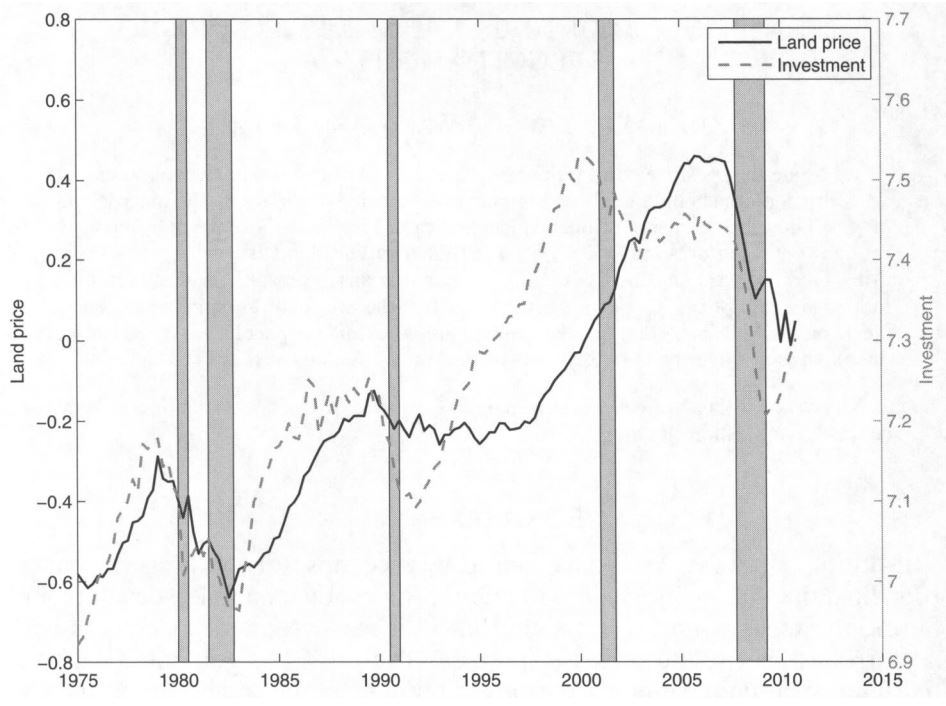
\includegraphics[width=0.8 \textwidth]{landpriceinvestment.JPG}
%    \end{tabular}
%    \caption{Real land price and investment (both in logs). Shaded areas are the NBER recession dates. Figure 1. from \cite{liu2013land}.}
%    \label{fig:landpriceinvestment}
%\end{figure}

\begin{figure}[h!]
    \centering
    \begin{tabular}{c}
        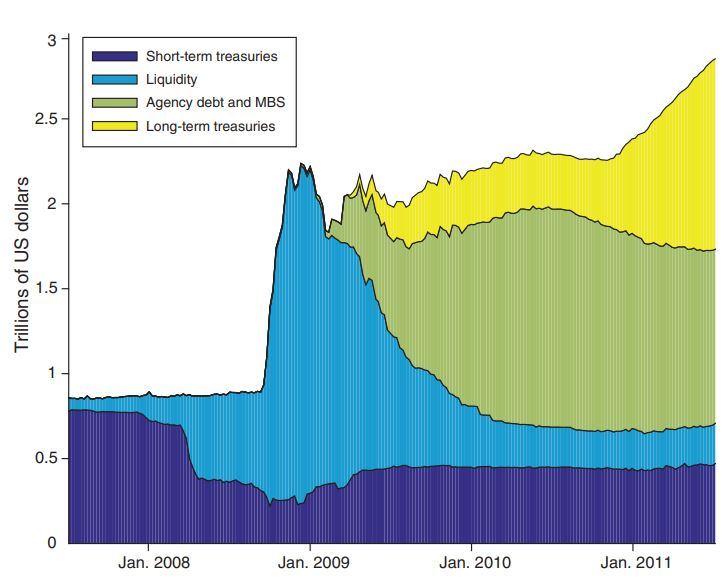
\includegraphics[width=0.8 \textwidth]{fedsheet.JPG}
    \end{tabular}
    \caption{federal Reserve's assets between July 2007 and July 2011.\\ Figure 1. from \cite{del2017great}}
    \label{fig:fedsheet}
\end{figure}

\end{document}

%------------------------------------------------------------------------------
% End of journal.tex
%------------------------------------------------------------------------------
